%%%%%%%%%%%%%%%%%%%%%%%%%%%%%%%%%%%%%%%%%%%%%%%%%%%%%%%%%%%%%%%%%%%%%
\newpage
\hfill 24.06.
%%%%%%%%%%%%%%%%%%%%%%%%%%%%%%%%%%%%%%%%%%%%%%%%%%%%%%%%%%%%%%%%%%%%%

\section{Denotationelle Semantik}


\begin{remark}[Ziel]
    Die Definition einer semantischen Funktion direkt ohne Umweg über eine simulierte Programmausführung (\dh{} ohne eine Übergangsrelation).

    Dabei ist die Zusammengsetztheit (\emph{compositionality}) bei der Definition der semantischen Funktion für ein Sprachkonstrukt wichtig, \dh{} man darf nur die Werte der semantischen Funktion für die Bestandteile des Sprachkonstrukts verwenden.
\end{remark}

\begin{example}
    \[ \A: \AExp \to \mathbb{Z}, \quad \B: \BExp \to \bool \]
    sind denotationell definiert.
\end{example}

\begin{example}[Gegenbeispiel]
    $\infruleNs[\true]{while}$: \[
        \frac{
            \strans{S}{\sigma}{\sigma''}, \strans{\texttt{while $b$ do $S$}}{\sigma''}{\sigma'}
        }{
            \strans{\underbrace{\texttt{while $b$ do $S$}}_{\text{gleiches Konstrukt}}}{\sigma}{\sigma'}
        }
    \]
\end{example}



\subsection{Direkte Definition der semantischen Funktion}

\begin{definition}
    Wir definieren $\mathcal{S}_{\text{ds}} : \Stm \to (\State \to \State)$.

    Die grundlegenden Definition bleiben gleich:
    \begin{align*}
        \Sdssem{\texttt{x := a}}(\sigma) & = \sigma[x \mapsto \Asem{a}(\sigma)] \\
        \Sdssem{\texttt{skip}}(\sigma) & = \sigma \\
        \Sdssem{\texttt{$S_1$; $S_2$}}(\sigma) & = (\underbrace{\Sdssem{S_2}}_{\State \to \State} \circ\;\, \Sdssem{S_1})(\sigma)
    \end{align*}

    \emph{Achtung:} Die Zustandsüberführungsfunktionen können eventuell nur partiell definiert sein. Dann liefert die Komposition auch nur $\bot$.

    Zur Definition von Verzweigungen ($\leadsto$ \texttt{if}) benutzen wir eine Hilfsfunktion \emph{cond} (siehe \defref{def:cond}). Damit ist die Definition von Verzweigungen wie folgt:
    \[
        \Sdssem{\texttt{if $b$ then $S_1$ then $S_2$}} = \cond(\Bsem{b}, \Sdssem{S_1}, \Sdssem{S_2})
    \]
\end{definition}

\begin{definition}[cond] \label{def:cond}
    \[
        \cond : (\State \to \bool) \times (\State \to \State) \times (\State \to \State) \to (\State \to \State)
    \]
    \[
        \cond(p, f_1, f_2) = \begin{cases}
            f_1(\sigma) & \text{falls } p(\sigma) = \true \\
            f_2(\sigma) & \text{falls } p(\sigma) = \false
        \end{cases}
    \]
\end{definition}

\par\bigskip
\emph{Herausforderung:} Definition von $\Sdssem{\texttt{while $b$ do $S$}}$ unter Berücksichtigung der Zusammengsetztheit.

\emph{Beobachtung:} \texttt{while $b$ do $S$} und \texttt{if $b$ then (S; while $b$ do $S$) else skip} sollen semantisch äquivalent sein.

Also eigentlich wollen wir schreiben: \[
    \Sdssem{\texttt{while $b$ do $S$}} = \cond(\Bsem{b}, \Sdssem{\underbrace{\texttt{while $b$ do $S$}}_{\text{gleiches Konstrukt}}} \;\circ\; \Sdssem{S}, \id)
\]
Das verletzt aber die Zusammengesetztheit.

\par\medskip
Wenn wir diese Gleichung betrachten, erkennen wir
\begin{remark}[Erkenntnis]
    $\Sdssem{\texttt{while $b$ do $S$}}$ ist die Lösung der Gleichung \[
        f = \cond(\Bsem{b}, f \circ \Sdssem{S}, \id)
    \]
\end{remark}

\emph{Wie lösen wir diese Gleichung?}



\subsubsection{Problemtransfer zu Fixpunkt eines Funktionals}

Wir überführen das Problem des Lösens der Gleichung zu einem Problem des Findens eines Fixpunktes.

\begin{definition}[Funktional] \label{def:funktional}
    Dafür definieren wir ein \emph{Funktional} (Argument und Ergebnis sind Funktionen): \[
        F : (\State \to \State) \to (\State \to \State)
    \] durch \[
        F(f) = \cond(\Bsem{b}, f \;\circ\; \Sdssem{S}, \id)
    \]
    Ein \emph{Fixpunkt} von $F$ ist ein $f^* : \State \to \State$ mit $F(f^*) = f^*$, \dh{} Stellen an denen die Funktion Werte auf sich selbst abbildet.
\end{definition}

Durch diese Herangehensweise, können wir die Funktion auch im Umfeld der Lösung betrachten oder sie benutzen, um sich der Lösung anzunähern.

\begin{definition}
    Wir definieren einen \emph{Fixpunktoperator} \[
        \fix : ((\State \to \State) \to (\State \to \State)) \to (\State \to \State)
    \]
    der einem Funktional $F$ einen Fixpunkt $f^*$ zuordnet.

    Dann können wir schreiben \[
        \Sdssem{\texttt{while $b$ do $S$}} = \fix(F)
    \]
    wobei \[
        F : f \mapsto \cond(\Bsem{b}, f \;\circ\; \Sdssem{S}, \id)
    \]
\end{definition}

Das heißt die Semantik der \texttt{while}-Schleife ist der Fixpunkt des Funktionals.

\begin{question}
    Was können wir über $\fix(f)$ sagen?
    \begin{enumerate}
        \item Existiert für \emph{jedes} Funktional $G : (\State \to \State) \to (\State \to \State)$ ein Fixpunkt?

            \textbf{Nein.}

            Betrachte $G$ mit \[
                G(g) = \begin{cases}
                    g_1 & \text{falls } g = g_2 \\
                    g_2 & \text{sonst}
                \end{cases}
            \]
            für $g_1 \neq g_2$.

            Aber vielleicht hat unser Funktional $F$ immer einen Fixpunkt.

        \item Falls es einen Fixpunkt gibt, ist dieser eindeutig?

            \textbf{Im Allgemeinen nein.}

            Betrachte $G$ mit \[ G(g) = g \] Hier sind alle $g$ Fixpunkte.

            Aber vielleicht hat unser Funktional $F$ immer höchstens einen Fixpunkt.
    \end{enumerate}
\end{question}

\par\bigskip
Wir müssen uns also anschauen, was der Fixpunktoperator $\fix$ mit unserem speziellen $F$ macht.

\begin{remark}[Intuition]
    Wie löst man eigentlich eine Fixpunkt-Gleichung $f = F(f)$?

    Fixpunktiteration: Start mit \begin{align*}
        f_0 & \\
        f_1 & = F(f_0) \\
        f_2 & = F(f_1) \\
        f_3 & = F(f_2) \\
        \dots
    \end{align*}
\end{remark}

\begin{example}[Kein Fixpunkt]
    \begin{align*}
        x & = 2x - 7 \\
        x_0 & = 20 \\
        x_1 & = 33 \\
        x_2 & = 59 \\
        x_3 & = 111 \\
        \dots
    \end{align*}
\end{example}


%%%%%%%%%%%%%%%%%%%%%%%%%%%%%%%%%%%%%%%%%%%%%%%%%%%%%%%%%%%%%%%%%%%%%
\newpage
\hfill 01.07.
%%%%%%%%%%%%%%%%%%%%%%%%%%%%%%%%%%%%%%%%%%%%%%%%%%%%%%%%%%%%%%%%%%%%%

\subsection{Der Fixpunktoperator}

\begin{remark}[Recap]
    Aus der letzten Vorlesung:

    \emph{Aufgabe:} Definiere die Semantik von \texttt{while $b$ do $S$} denotationell.

    \emph{Idee:} Betrachte Funktional $F$ (siehe \defref{def:funktional}). Dann sollte die Zustands"-über"-führungs"-funktion ein Fixpunkt von $F$ sein, \dh{} $f^* = F(f^*)$.
\end{remark}

\par\bigskip
\begin{question}
    Woher wissen wir, dass $F$ einen Fixpunkt besitzt? Wie sieht dieser Fixpunkt aus?
\end{question}

\par\bigskip
Versuch einer Visualisierung:

Wir haben $\Bsem{b}$ (Punkte sind Zustände mit Wahrheitswerten) und $\Ssem{S}$ (partielle Zustandsüberführungsfunktion, gelb), eine Funktion (Kandidat für Fixpunkt, blau) und das $f$-Funktional $F(f)$ (grün).

$F$ erzeugt also eine neue Zustandsüberführungsfunktion, die für Zustände mit $\false$ auf den Zustand selbst abbildet und für Zustände mit $\true$ durch $f \circ \mathcal{S}$ abbildet, \dh{} erst dem gelben, dann dem blauen Pfeil folgt.

Die Aufgabe des Findens eines Fixpunktes bedeutet also, ein $f$ (blau) zu finden, sodass nach Anwendung von $F(f)$ (grün) die gleichen Pfeile entstehen wie in $f$.
\begin{figure}[H]
    \centering
    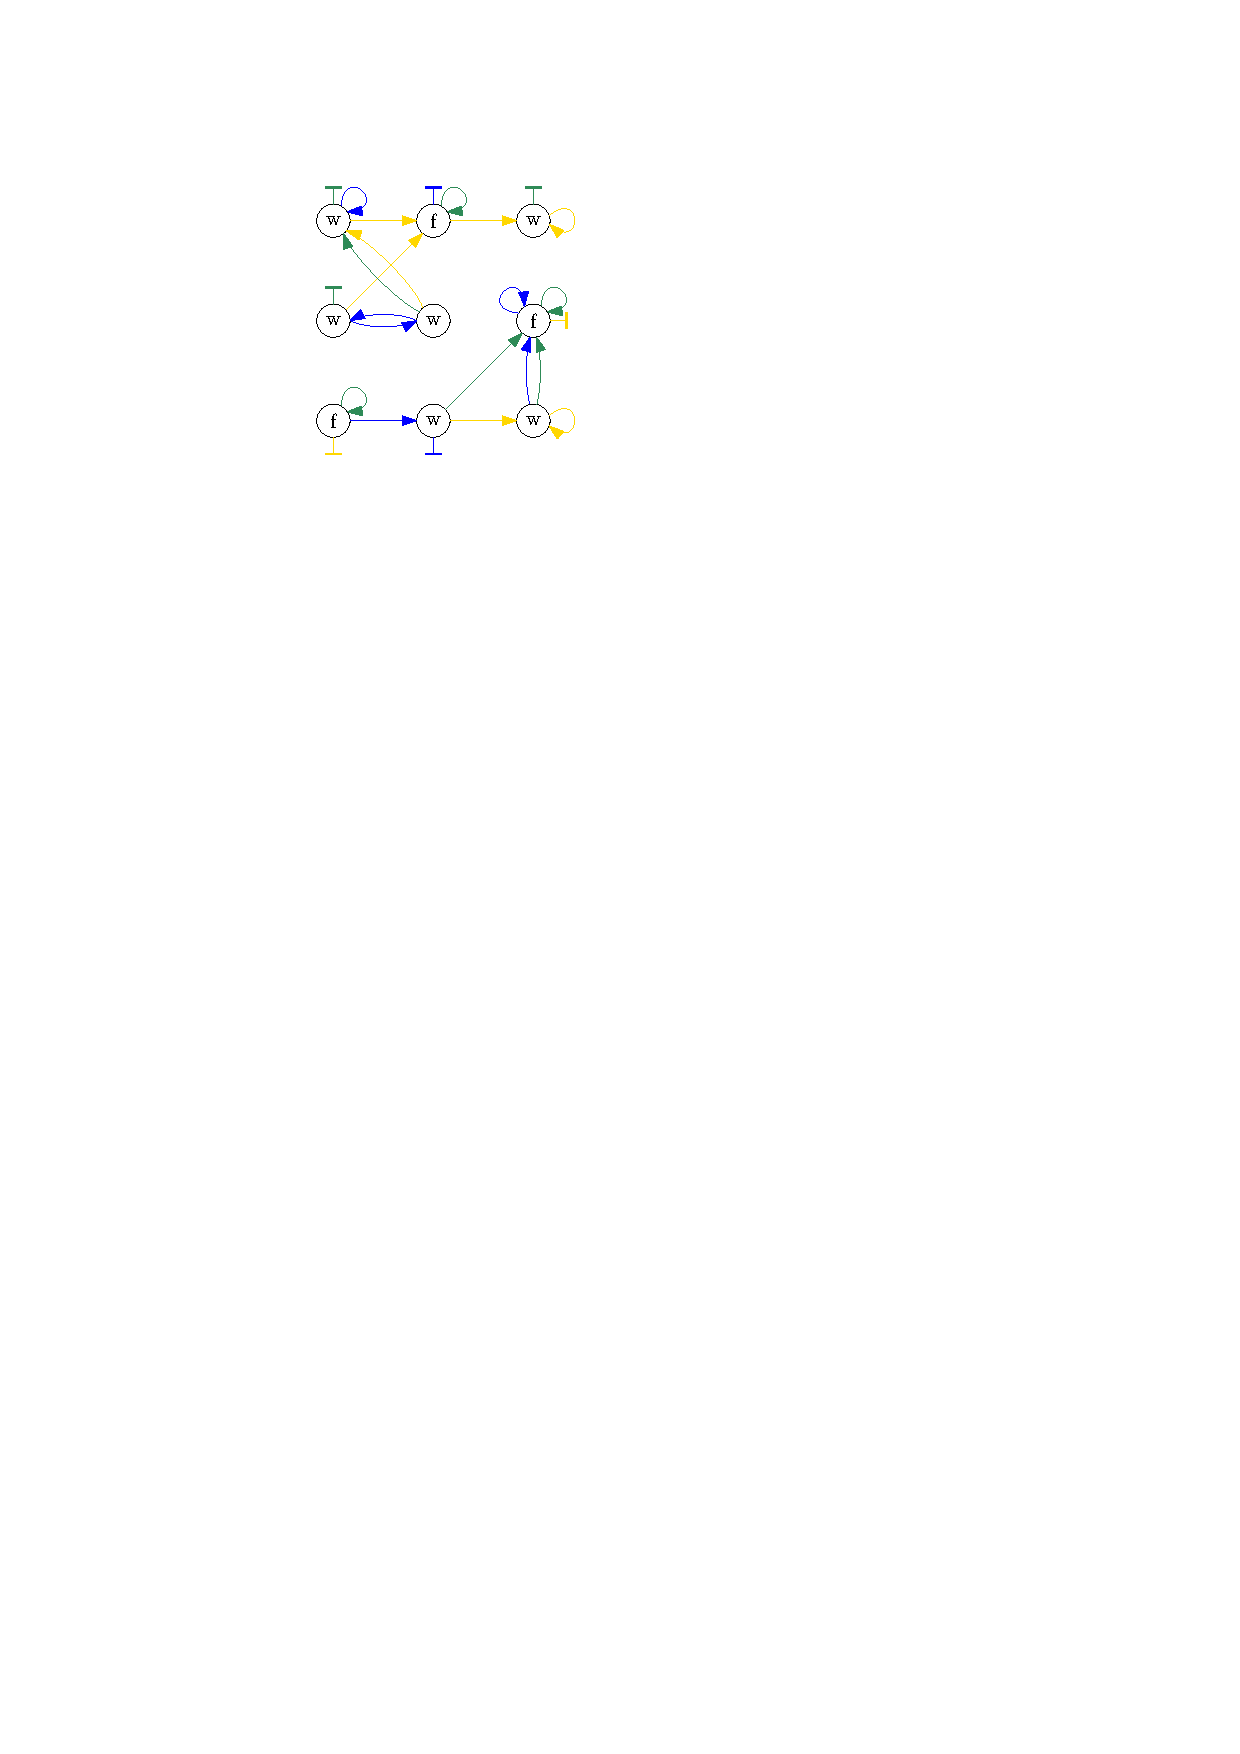
\includegraphics[page=1,width=.4\textwidth]{img/f-combined}
    \caption{Visualisierung der Funktionsverkettung durch $F$}
\end{figure}



\subsubsection{Wie muss ein Fixpunkt aussehen?}

\begin{enumerate}
    \item Für alle Zustände mit Wahrheitswert $\false$ muss der Fixpunkt eine Schleife ($\id$) liefern.
        \begin{figure}[H]
            \centering
            \includegraphics[page=2,width=.15\textwidth]{img/f-combined}
        \end{figure}
    \item Es gibt Zustände mit Wahrheitswert $\true$, die nach endlich vielen Schritten mit $\mathcal{S}$ (gelb) einen Zustand mit Wahrheitswert $\false$ erreichen.
        \begin{figure}[H]
            \centering
            \includegraphics[page=3,width=.6\textwidth]{img/f-combined}
        \end{figure}
    \item Es gibt Zustände mit Wahrheitswert $\true$, die nicht nach endliche vielen Schritten einen Zustand mit Wahrheitswert $\false$ erreichen.
        \begin{enumerate}
            \item $w \to w \to w \to \dots$
\begin{lstlisting}[language=Pascal]
x := 1;
while true do
    x := x + 1
\end{lstlisting}
                \begin{figure}[H]
                    \centering
                    \includegraphics[page=4,width=.6\textwidth]{img/f-combined}
                \end{figure}
                Hier müssen alle Pfeile zum selben Zustand zeigen, egal welcher genau das ist.
            \item  $w_0 \to w_1 \to w_2 \to w_3 \to w_0$
\begin{lstlisting}[language=Pascal]
x := 0;
while x != -1 do
    x := (x + 1) mod 4
\end{lstlisting}
                \begin{figure}[H]
                    \centering
                    \includegraphics[page=5,width=.22\textwidth]{img/f-combined}
                \end{figure}
                Hier müssen ebenfalls alle Pfeile zum selben Zustand zeigen, egal welcher genau das ist.
            \item $w \to w \to w \to \bot$
\begin{lstlisting}[language=Pascal]
x := 1;
while x < 20 do
    x := x + 1;
    if x = 10 then
        while true do skip
    else
        ...
\end{lstlisting}
        \begin{figure}[H]
            \centering
            \includegraphics[page=6,width=.6\textwidth]{img/f-combined}
        \end{figure}
        \end{enumerate}
        Für die Fälle (a) und (b) ist der Fixpunkt also fix aber beliebig (inklusive $\bot$).
\end{enumerate}

\par\bigskip
Das Ergebnis unserer informellen Überlegung ist:
\begin{itemize}
    \item Wir erwarten, dass \emph{immer ein Fixpunkt existiert}.
    \item Ein solcher Fixpunkt ist nicht immer eindeutig. Für Zustände, bei denen die \texttt{while}-Schleife nicht terminiert, kann es ggf. mehrere Möglichkeiten für einen Fixpunkt geben.

        In diesem Fall hätten wir gern den Fixpunkt, der $\bot$ für nicht-terminierende Schleifen liefert.
\end{itemize}


\subsubsection{Fixpunktiteration}

\begin{remark}[Idee]
    Finde den richtigen Fixpunkt durch Fixpunktiteration. Starte mit der Zustandsüberführungsfunktion \[
    f_{\bot} : f_{\bot}(\sigma) = \bot \quad \forall \sigma \in \State
    \]
    welche $F$ wiederholt auf $f_{\bot}$ an, schaue was passiert.

    $\Rightarrow$ Der ``Grenzwert'' ist der gewünschte Fixpunkt.

    Z.\,B. bei (c.a) und (c.b) bleibt die Funktion nach wiederholter Anwendung überall $\bot$.
\end{remark}

\begin{definition}[Fixpunktoperator]
    \begin{align*}
        f_0 & = f_{\bot} \\
        f_n &= F(f_{n-1}) \quad n \geq 1 \\
        \fix(f) & := \lim_{n \to \infty} f_n
    \end{align*}

    Aber wie ist der Grenzwert in diesem Kontext definiert?
\end{definition}



\subsection{Relationen und Ordnungen}

\begin{definition}
    Sei $\mathcal{F} = \{ f \;\vert\; f: \State \to \State \}$ die Menge aller \emph{partiellen} Zustandsüberführungsfunktionen. Wir definieren auf $\mathcal{F}$ eine Relation $\sqsubseteq$ durch \[
        f \sqsubseteq g :\Longleftrightarrow \forall \sigma, \sigma' \in \State: f(\sigma) = \sigma' \Rightarrow g(\sigma) = \sigma'
        \]
        \dh{} überall, wo $f$ definiert ist, ist auch $g$ definiert und liefert denselben Wert.
\end{definition}

\par\medskip
\begin{example}
    $g_1, g_2, g_3, g_4 : \State \to \State$
    \begin{align*}
        g_1(\sigma) & = \sigma \quad \forall \sigma \in \State \\
        g_2(\sigma) & = \begin{cases}
            \sigma & \text{falls } \sigma(x) \geq 0 \\
            \bot & \text{sonst} \\
        \end{cases} \\
        g_3(\sigma) & = \begin{cases}
            \sigma & \text{falls } \sigma(x) \leq 0 \\
            \bot & \text{sonst} \\
        \end{cases} \\
        g_4(\sigma) & = \begin{cases}
            \sigma & \text{falls } \sigma(x) = 0 \\
            \bot & \text{sonst} \\
        \end{cases} \\
    \end{align*}
    Behauptung:
    \begin{align*}
        g_4 \sqsubseteq g_2 \sqsubseteq g_1 \\
        g_4 \sqsubseteq g_3 \sqsubseteq g_1 \\
        g_4 \sqsubseteq g_1 \tag{*}
    \end{align*}
    $(*)$ folgt aus Transitivität da die Relation eine Ordnungsrelation ist, aber das haben wir noch nicht bewiesen.

    Jedoch sind $g_2$ und $g_3$ nicht vergleichbar.
\end{example}

\par\bigskip
\begin{remark}[Fakt]
    $\sqsubseteq$ ist eine Ordnungsrelation auf $\mathcal{F}$. Das bedeutet, sie ist
    \begin{itemize}
        \item reflexiv: $f \sqsubseteq f$
        \item transitiv: $f \sqsubseteq g \wedge g \sqsubseteq h \Rightarrow f \sqsubseteq h$
        \item antisymmetrisch: $f \sqsubseteq g \wedge g \sqsubseteq f \Rightarrow f = g$
    \end{itemize}

    $(\mathcal{F}, \sqsubseteq)$ ist eine \emph{Halbordnung} (poset bzw. partially ordered set).
\end{remark}

\par\medskip
\begin{definition}
    Ein Element $f \in \mathcal{F}$ heißt \emph{Minimum}, falls für alle $g \in \mathcal{F}$ gilt \[
    f \sqsubseteq g
    \]
\end{definition}

\begin{observations}
    Im Allgemeinen, muss es kein Minimum in einem poset geben (\zb{} unendliche Ordnung oder mehrere nicht vergleichbare minimale Elemente). Wenn ein \emph{Minimum} existiert, dann ist es \emph{eindeutig} (wegen Antisymmetrie).

    Aber $(\mathcal{F}, \sqsubseteq)$ hat ein Minimum und zwar $f_{\bot}$.
\end{observations}



%%%%%%%%%%%%%%%%%%%%%%%%%%%%%%%%%%%%%%%%%%%%%%%%%%%%%%%%%%%%%%%%%%%%%
\newpage
\hfill 08.07.
%%%%%%%%%%%%%%%%%%%%%%%%%%%%%%%%%%%%%%%%%%%%%%%%%%%%%%%%%%%%%%%%%%%%%

\begin{remark}[Ziel für den Rest der Vorlesung]
    Konvergenz der Fixpunktiteration beweisen.
\end{remark}

\begin{definition}[Obere Schranke, Supremum]
    Sei $\mathcal{G} \subseteq \mathcal{F}$, dann ist auch $(\mathcal{G}, \sqsubseteq)$ eine Halbordnung.

    Ein Element $f \in \mathcal{F}$ heißt \emph{obere Schranke} von $\mathcal{G}$, falls \[
        \forall g \in \mathcal{G}: g \sqsubseteq f
    \]

    Eine obere Schranke von $\mathcal{G}$ heißt \emph{Supremum} ``$\sup \mathcal{G}$'', falls für alle oberen Schranken $f'$ von $\mathcal{G}$ gilt $f \sqsubseteq f'$ \dh{} es ist die kleinste obere Schranke.

    Falls ein \emph{Supremum} existiert, so ist es \emph{eindeutig}. Falls die obere Schranke innerhalb von $\mathcal{G}$ liegt, so ist sie auch das Maximum und Supremum von $\mathcal{G}$.
\end{definition}

\par\bigskip
\begin{definition}
    Sei $\mathcal{G} \subseteq \mathcal{F}$. Wir nennen $\mathcal{G}$ eine \emph{Kette} (chain), falls $\mathcal{G}$ total geordnet ist, \dh{} \[
        \forall g_1, g_2 \in \mathcal{G}: g1 \sqsubseteq g_2 \vee g_2 \sqsubseteq g_1
    \]
\end{definition}

\begin{example}
    Folgende Beispiele sind Ketten:
    \begin{itemize}
        \item Die leere Menge $\varnothing \subseteq \mathcal{F}$ ist eine Kette.
        \item Jede 1-elementige Menge ist eine Kette.
        \item Sei $x \in \Var$ eine Variable. Für $n \in \mathbb{N}$ definiere wir $g_n \in \mathcal{F}$ durch \begin{align*}
                g_n: & \State \to \State \\
                g_n(\sigma) & = \begin{cases}
                    \bot & \text{falls } \sigma(x) > n \\
                    \sigma[x \mapsto -1] & \text{falls } \sigma(x) \in \{ 0, \dots, n \} \\
                    \sigma & \text{falls } \sigma(x) < 0
                \end{cases}
            \end{align*}
            Die Menge $\{ g_n \mid n \in \mathbb{N} \}$ ist eine Kette in $(\mathcal{F}, \sqsubseteq)$, denn es gilt \[
                    g_n \sqsubseteq g_m \Leftrightarrow n \leq m
                \]
\begin{lstlisting}[escapeinside={/*}{*/}, language=Pascal, caption=Snippet für $g_n$]
while x >= 0 do  /*\label{code:loopdec}*/
    x := x - 1
\end{lstlisting}
            % TODO: foto
            \emph{Ziel:} Die Funktion \begin{align*}
                g_{\infty}: & \State \to \State \\
                g_{\infty} & = \begin{cases}
                    \sigma[x \mapsto -1] & \text{falls } \sigma(x) \geq 0 \\
                    \sigma & \text{sonst}
                \end{cases}
            \end{align*}
            ist die Semantik von Listing~\ref{code:loopdec}.

            Nun sehen wir, dass \[
                g_{\infty} = \sup \{ g_n \mid n \in \mathbb{N} \}
            \]
    \end{itemize}
\end{example}

\par\bigskip
\begin{definition}[Kettenvollständigkeit]
    Eine Halbordnung heißt \emph{kettenvollständig} (ccpo: chain-complete-partial order), falls jede Kette ein Supremum besitzt.
\end{definition}

\par\medskip
\begin{example}
    $(\mathbb{N}, \leq)$ ist nicht kettenvollständig. Die Menge der geraden Zahlen $\{ 2, 4, \dots \}$ ist eine Kette ohne Supremum.

    \par\medskip
    $(\mathcal{P}(\{ 1, 2, 3 \}), \subseteq)$ ist kettenvollständig.
    \begin{figure}[H]
        \centering
        % https://tex.stackexchange.com/questions/584458/drawing-a-hasse-diagram-in-latex
        \begin{tikzcd}[row sep=1.5cm, column sep=1.7cm]
                             & \{1,2,3\} \\
            \{1,2\}\urar       & \{1,3\}\uar \arrow[from=dr]                        & \{2,3\}\ular \\
            \{1\}\uar\urar & \{2\}\ular[crossing over] \urar[crossing over] & \{3\}\uar\\
                             & \varnothing \ular\uar\urar
        \end{tikzcd}
        \caption{Hasse-Diagramm für $(\mathcal{P}(\{1,2,3\}), \subseteq)$}
    \end{figure}

    \par\medskip
    $(\mathcal{P}(\mathbb{N}), \subseteq)$ ist auch kettenvollständig. Sei $X \in (\mathcal{P}(\mathbb{N}), \subseteq)$ eine Kette, also eine Menge von Teilmengen von $\mathbb{N}$, sodass $\forall A, B \in X: A \subseteq B \vee B \subseteq A$.\\
    Es ist $\sup X = \bigcup_{A \in X} A = Z$, da \begin{enumerate}
        \item Sei $A = X$. Dann ist $A \subseteq Z$.
        \item $Z$ ist kleinste obere Schranke. Sei $Y$ obere Schranke von $X$.

            Zu zeigen: $Z \subseteq Y$.

            Nimm $z \in Z$, zeige, dass $z \in Y$.
            \begin{align*}
                z \in Z \Rightarrow \exists A \subseteq Z \text{ mit } z \in A
            \end{align*}
            Da $Y$ obere Schranke von $X$ ist und $a \in X$, muss $A \subseteq Y$. Also folgt, $z \in Y$.
    \end{enumerate}
\end{example}

\par\bigskip
\begin{remark}[Fakt]
    Sei $(\mathcal{D}, \sqsubseteq)$ ccpo. Dann besitzt $\mathcal{D}$ ein Minimum, nämlich \[
            d_{\bot} = \sup \varnothing
        \]
\end{remark}

\begin{proof}
    Sei $d_{\bot} = \sup \varnothing$. $d_{\bot}$ existiert nach Annahme. Und sei $d \in \mathcal{D}$. Nach Definition ist $d$ eine obere Schranke von $\varnothing$. Da $d_{\bot} = \sup \varnothing$, muss $d_{\bot} \sqsubseteq d$ sein, \dh{} $d_{\bot}$ ist Minimum.
\end{proof}

\par\bigskip
\begin{theorem} \label{theorem:fkette}
    $(\mathcal{F}, \sqsubseteq)$ ist kettenvollständig.

    Sei $\mathcal{G} \subseteq \mathcal{F}$ eine Kette. Dann ist $\sup \mathcal{G}$ die Funktion mit \[
        \graph(\sup \mathcal{G}) = \bigcup \, \{ \graph(g) \mid g \in \mathcal{G} \}
    \]
    \dh{} \[
        (\sup \mathcal{G})(\sigma) = \sigma' \Leftrightarrow \exists g \in \mathcal{G}: g(\sigma) = \sigma'
    \]
\end{theorem}

\begin{proof}
    Wir müssen die folgenden Eigenschaften beweisen:
    \begin{enumerate}
        \item Wohldefiniertheit

            Seien $g_1, g_2 \in \mathcal{G}$ und sei $\sigma \in \State$, sodass $g_1(\sigma) \neq \bot \neq g_2(\sigma)$. Da $\mathcal{G}$ eine Kette ist, muss gelten $g_1 \sqsubseteq g_2 \vee g_2 \sqsubseteq g_1$. In beiden Fällen folgt $g_1(\sigma) = g_2(\sigma)$. Also ist der Wert von $(\sup \mathcal{G})(\sigma)$ wohldefiniert.
        \item obere Schranke

            Aus der Definition folgt direkt, dass $(\sup \mathcal{G})$ eine obere Schrank ist: \[
                g \in \mathcal{G}, \; \sigma, \sigma' \in \State, \; g(\sigma) = \sigma' \implies (\sup \mathcal{G})(\sigma) = \sigma'
            \]
        \item kleinste obere Schranke

            $(\sup \mathcal{G})$ ist obere Schranke. Sei $h$ eine obere Schranke.

            Zu zeigen: $(\sup \mathcal{G}) \sqsubseteq h$.

            Sei $\sigma, \sigma' \in \State$. $(\sup \mathcal{G})(\sigma) = \sigma'$, \dh{} $\exists g \in \mathcal{G}: g(\sigma) = \sigma'$, \dh{} $h$ ist obere Schranke, \dh{} $g \sqsubseteq h$, also muss $h(\sigma) = \sigma'$.
    \end{enumerate}
\end{proof}

Idee der Fixpunktiteration: \begin{align*}
    f_0 & = f_{\bot} \\
    f_1 & = F(f_0) \\
    \vdots \\
    f_{\infty} & = \sup \, \{ f_n \mid n \in \mathbb{N} \}
\end{align*}
Dann soll gelten: $f_{\infty} = F(f_{\infty})$.

Wenn also gelten würde \[
    F\left(\lim_{n \to \infty} f_n\right) = \lim_{n \to \infty} F(f_n)
\] wären wir fertig. Das ist die \emph{Stetigkeit}.



%%%%%%%%%%%%%%%%%%%%%%%%%%%%%%%%%%%%%%%%%%%%%%%%%%%%%%%%%%%%%%%%%%%%%
\newpage
\hfill 15.07.
%%%%%%%%%%%%%%%%%%%%%%%%%%%%%%%%%%%%%%%%%%%%%%%%%%%%%%%%%%%%%%%%%%%%%

\begin{remark}[Letztes Mal]
    Satz~\ref{theorem:fkette}: $(\mathcal{F}, \sqsubseteq)$ ist kettenvollständig.

    Was bisher fehlt ist ein in Konzept von Stetigkeit, sodass man Folgendes schreiben kann: \[
        \lim_{n \to \infty} f(x_n) = f\left(\lim_{n \to \infty} x_n\right)
    \]
\end{remark}


\par\medskip
\begin{definition}[Monotonie]
    Eine totale Funktion $f: D \to Z$ heißt \emph{monoton}, falls für alle $d_1, d_2 \in D$ gilt \[
        d_1 \sqsubseteq d_2 \Rightarrow f(d_1) \sqsubseteq' f(d_2)
    \]
\end{definition}

\begin{observations}
    Wir beobachten folgende Eigenschaften:
    \begin{enumerate}
        \item Seien $(\mathcal{D}, \sqsubseteq), (\mathcal{D}',\sqsubseteq'), (\mathcal{D}'',\sqsubseteq'')$ ccpos und $f_1: \mathcal{D} \to \mathcal{D}'$ und $f_2: \mathcal{D}' \to \mathcal{D}''$ monoton Funktionen.

            Dann ist auch $f_1 \circ f_2$ monoton.
        \item Seien $(\mathcal{D}, \sqsubseteq), (\mathcal{D}',\sqsubseteq')$ ccpos und $f: \mathcal{D} \to \mathcal{D}'$ eine monotone Funktion. Sei $\mathcal{K}$ eine Kette. Dann ist $f(\mathcal{K})$ eine Kette in $\mathcal{D}'$. Wenn $\mathcal{D}$ endlich ist, dann ist das Supremum von $\mathcal{D}'$: \[
                \sup' \mathcal{D}' = f(\sup \mathcal{D})
            \]

            Im Allgemeinen gilt: $f(\sup S) \sqsubsetneqq' \sup' f(S)$
    \end{enumerate}
\end{observations}


\par\bigskip
\begin{definition}[Stetigkeit]
    Seien $(\mathcal{D}, \sqsubseteq), (\mathcal{D}',\sqsubseteq')$ ccpos und $f: \mathcal{D} \to \mathcal{D}'$ heißt \emph{stetig} wenn:
    \begin{enumerate}
        \item $f$ ist monoton.
        \item Für alle nichtleeren Ketten $\mathcal{S} \in \mathcal{D}$ gilt $\sup' f(\mathcal{S}) = f(\sup\, \mathcal{S})$.
    \end{enumerate}
\end{definition}

\par\medskip
\begin{observation}
    Seien $(\mathcal{D}, \sqsubseteq), (\mathcal{D}',\sqsubseteq'), (\mathcal{D}'',\sqsubseteq'')$ ccpos und seien die beiden Funktionen $f: \mathcal{D} \to \mathcal{D}'$ und $f': \mathcal{D}' \to \mathcal{D}''$ stetig.

    Dann ist $f' \circ f: \mathcal{D} \to \mathcal{D}''$ stetig.
\end{observation}


\par\bigskip
\begin{theorem}
    Sei $(\mathcal{D}, \sqsubseteq)$ ccpo mit Minimum $d_h$ und sei $F : \mathcal{D} \to \mathcal{D}$ eine stetige Funktion. Setze $f_0 = d_{\bot}$ und $f_n = f(f_{n-1})$.

    \begin{enumerate}
        \item Dann ist $\{ f_n \mid n \in \mathbb{N} \}$ eine Kette.
        \item Sei $\fix(F) = \sup \{ f_n \mid n \in \mathbb{N} \}$. Dann gilt $F(\fix(F)) = \fix(F)$.
        \item Außerdem gilt $\forall g \in \mathcal{D}, F(g) = g: g \geq \fix(F)$.
    \end{enumerate}
\end{theorem}

\begin{proof}
    Wir führen den Beweis stückweise.
    \begin{enumerate}
        \item $\{ f_n \mid n \in \mathbb{N} \}$ ist eine Kette. \\
            Seien $f_n, f_m$ mit $m > n$. Zu zeigen $f_n \sqsubseteq f_m$.

            Setze $a = n - m > 0$. Da $f_0 = d_{\bot}$ Minimum ist, gilt $f_0 \sqsubseteq f_a$. Da $F$ stetig ist, folgt
            \begin{align*}
                F(f_0) & \sqsubseteq F(f_n) \\
                \Rightarrow f_1 & \sqsubseteq f_{a+1} \\
                & n\text{-mal} \dots \\
                \Rightarrow f_n & \sqsubseteq f_{a+n}
            \end{align*}

        \item $\fix(F)$ ist Fixpunkt von $F$.
            \begin{align*}
                F(\fix(F)) & = F(\sup \{f_n \mid n \in \mathbb{N} \}) \tag{Def} \\
                & = \sup F(\{f_n \mid n \in \mathbb{N} \}) \tag{Stetigkeit} \\
                & = \sup \{F(f_n) \mid n \in \mathbb{N} \} \\
                & = \sup \{f_{n+1} \mid n \in \mathbb{N} \} \tag{Def} \\
                & = \sup (\{f_{n+1} \mid n \in \mathbb{N} \} \cup \{ d_{\bot} \}) \tag{Minimum} \\
                & = \fix(F) \tag{Def}
            \end{align*}

        \item $\fix(f)$ ist minimaler Fixpunkt.

            Sei $g \in \mathcal{D}$ und $F(g) = g$. Es gilt $g \sqsupseteq d_{\bot}$ ($d_{\bot}$ ist Minimum).

            Also auch $F(g) \sqsupseteq F(d_{\bot})$ bzw. $g \sqsupseteq f_1$. Also auch $F(g) \sqsupseteq F(f_1)$ bzw. $g \sqsupseteq f_2$ usw.

            Also gilt nach Induktion $g \sqsupseteq f_n, n \in \mathbb{N}$. $g$ ist eine obere Schranke von $\{f_n \mid n \in \mathbb{N} \}$. Nach Definition vom Supremum, ist $g$ die kleinste obere Schranke.
            \[ \fix(f) = \sup \{ f_n \mid n \in \mathbb{N} \} \sqsubseteq g \]
    \end{enumerate}
\end{proof}

\par\medskip
\emph{Zurück zum ursprünglichem Ziel:} Nun möchten wir schreiben: \[ \Sdssem{\texttt{while $b$ do $S$}} = \fix(F)
\] wobei $F(g) = \cond(\Bsem{b}, g \circ \Sdssem{S}, \id)$ und $f \circ g: \State \to \State$.


Nach dem Satz müssen wir jetzt nur noch überprüfen, dass $F$ stetig ist.
Das funktioniert so: Wir beobachten, dass sich $F$ schreiben lässt als $F = F_2 \circ F_1$, wobei $F_1(g) = g \circ \Sdssem{S}$
und $F_2(g) = \cond(\Bsem{b}, g, \id)$.

$\Sdssem{\cdot}$ ist schwierig, also beweisen wir die Stetigkeit getrennt.

\begin{proof}[Skizze]
    Zu zeigen:
    \begin{enumerate}
        \item $F_2$ ist stetig, durch detaillierte Analyse.
        \item $F_1$ ist stetig. Beobachtung: Für jedes feste $g_0: \State \to \State$:

            Ist $F_1(f) = f \circ g_0$ stetig?
    \end{enumerate}
    $\Rightarrow F_2 \circ F_1$ ist stetig.
\end{proof}


\begin{theorem}
    $\Sdssem{\cdot}$ definiert eine semantische Funktion auf der Menge aller \texttt{while}-Programme.
\end{theorem}

\begin{proof}[Skizze]
    Durch strukturelle Induktion nach der Anweisung $S$.
\end{proof}



\subsection{Eigenschaften der denotationellen Semantik}

Seien $S_1, S_2$ Anweisungen. Wir sagen, sie sind semantisch äquivalent, wenn \[
    \Sdssem{S_1} = \Sdssem{S_2}
\] (Vergleich als mathematische Funktionen).

\par\medskip
\begin{example}
    $S$ und $S; \texttt{skip}$ sind semantisch äquivalent.

    \begin{align*}
        \Sdssem{S_1} & = \Sdssem{S_1; \texttt{skip}} \\
        & =\Sdssem{\texttt{skip}} \circ \Sdssem{S_1} \\
        & = \id \circ \; \Sdssem{S_1} \\
        & = \Sdssem{S_1} \quad \checkmark
    \end{align*}

    oder auch \[
        S_1; (S_2; S_3) \text{ und } (S_1; S_2); S_3
    \] durch Assoziativität der Funktionskomposition. Und auch \[
        \texttt{while $b$ do $S$} \text{ und } \texttt{if $b$ then ($S$; while $b$ do $S$) else skip}
    \]
\end{example}


\begin{theorem}
    Sei $S$ eine Anweisung in der \texttt{while}-Sprache, dann gilt: \[
        \Sdssem{S} = \Ssossem{S}
    \]
\end{theorem}

\begin{proof}[Skizze]
    Durch Fallunterscheidung/Induktion.

    Der Beweis verwendet die Antisymmetrie von $(\mathcal{F}, \sqsubseteq)$. Wir zeigen, dass \[
        \Sdssem{\cdot} \sqsubseteq \Ssossem{\cdot} \text{ und } \Ssossem{\cdot} \sqsubseteq \Sdssem{\cdot}
    \]

    \begin{enumerate}
        \item $\Ssossem{\cdot} \sqsubseteq \Sdssem{\cdot}$ \\
            Sei $S$ eine Anweisung, dann gilt $\Ssossem{\cdot} \sqsubseteq \Sdssem{\cdot}$, \dh{} für alle $\sigma, \sigma'$ gilt:
            Falls $\Ssossem{S}(\sigma) = \sigma'$, dann auch $\Sdssem{S}(\sigma) = \sigma'$.

            Nach Definition gilt \[
                \Ssossem{S}(\sigma) = \sigma' \Longleftrightarrow \langle S, \sigma \rangle \Rightarrow^* \sigma'
            \]
            Dann zeigen wir: Wenn $\langle S, \sigma \rangle = \sigma'$, dann gilt $\Sdssem{S}(\sigma)=\sigma'$.
            Und wenn gilt $\langle S, \sigma \rangle = \langle S', \sigma' \rangle$, dann gilt $\Sdssem{S}(\sigma) = \Sdssem{S'}(\sigma')$.

        \item $\Sdssem{\cdot} \sqsubseteq \Ssossem{\cdot}$ \\

            Sei $S$ eine Anweisung, dann gilt $\Sdssem{\cdot} \sqsubseteq \Ssossem{\cdot}$. Also gilt \[
                    \Sdssem{S}(\sigma) = \sigma' \implies \Ssossem{S}(\sigma) \Rightarrow^* \sigma'
            \]
            Beweis: Strukturelle Induktion und Definition des Fixpunktoperators (Beweis ist lang).
    \end{enumerate}
\end{proof}



%%%%%%%%%%%%%%%%%%%%%%%%%%%%%%%%%%%%%%%%%%%%%%%%%%%%%%%%%%%%%%%%%%%%%
\newpage
\hfill 22.07.
%%%%%%%%%%%%%%%%%%%%%%%%%%%%%%%%%%%%%%%%%%%%%%%%%%%%%%%%%%%%%%%%%%%%%

\subsection{Programmanalyse mit denotationeller Semantik}

\emph{Ziel:} Erhalte Informationen über das \emph{dynamische} Verhalten eines Programms durch eine \emph{statische} Analyse ohne das Programm auszuführen, \zb{} mit \texttt{lint} für die Sprache C.

\begin{example}
    Verschiedene Anwendungen für statische Programmanalyse:
    \begin{itemize}
        \item definition-use-Analyse: Sind Variablen initialisiert bevor sie benutzt werden?
        \item constant-propagation: Werte/Ausdrücke, im Vorhinein auswerten, die nicht vom Zustand des Programms abhängen.
        \item Intervall-Analyse: Bestimme Intervalle für mögliche Variablenwerte.
    \end{itemize}

\end{example}

\emph{Hier:} Sonderfall der Intervall-Analyse: \emph{Vorzeichenanalyse}, \dh{} bestimme statisch mögliche Vorzeichen für die Variablen im Programm.



\subsubsection{Vorzeichenanalyse}

\emph{Idee:} Arbeite mit Funktionen, die Eigenschaften von Zuständen abbilden und nicht die Zustände selbst (\emph{property states}). Dazu benötigen wir die Menge abstrakter Eigenschaften von Programmvariablen $\mathcal{P}$.

\par\medskip
\begin{definition} \label{def:vorzeichenanalyse}
    \[
    \mathcal{P} = \{ \text{POS}, \text{NEG}, \text{NULL}, \text{BEL} \}
    \]
    wobei BEL ``beliebig'' bedeutet.

    Wir definieren außerdem eine partielle Ordnung $\sqsubseteq_{\mathcal{P}}$ auf $\mathcal{P}$ mit der Bedeutung ``$p_1 \sqsubseteq_{\mathcal{P}} p_2$'': $p_1$ ist mindestens so spezifisch wie $p_2$, \zb{} POS $\sqsubseteq_{\mathcal{P}}$ BEL.

    Wir nehmen an, dass $\sqsubseteq_{\mathcal{P}}$ so definiert ist, dass alle Teilmengen $Y \subseteq \mathcal{P}$ ein Supremum besitzen (\emph{vollständiger Verband}). Dann gibt das Supremum die allgemeinste Eigenschaft einer Menge von Eigenschaften an.
\end{definition}

In der Programmanalyse arbeiten wir mit \emph{abstrakten Zustandseigenschaften} (property states), die jeder Variable eine Eigenschaft zuordnen statt eines konkreten Wertes: \[
    \PState: \Var \to \mathcal{P}
\]

\begin{lemma}
    Wenn $\mathcal{P}$ ein vollständiger Verband ist (siehe \defref{def:vorzeichenanalyse}), dann gilt das auch für $\PState$.

    Genaue Formulierung nicht hier \dots
\end{lemma}

\par\bigskip
\emph{Idee:} Bisher hatten wir $\mathcal{S} : \Stm \to (\State \to \State)$. Nun betrachten wir die Analysefunktion $\mathcal{DS}: \Stm \to (\PState \to \PState)$.

\begin{remark}[Halteproblem]
    Wir können nicht erwarten, dass die Programmanalyse immer die genauest mögliche Antwort liefert.

\begin{lstlisting}[language=Pascal]
y := 1;
if bla then
    x := 1;
else
    S;
    x := -1;
y := x
\end{lstlisting}

    Hier hängt die Vorzeichenanalyse für $y$ davon ab, ob $S$ terminiert oder nicht, \dh{} unsere Analyse ist notwendigerweise approximativ und wird sagen, dass $y$ negativ sein könnte.
\end{remark}



\subsubsection{Vorzeichenanalyse von \texttt{while}}

\begin{enumerate}
    \item Wir definieren die gewünschte Eigenschaft, \dh{} eine Variable ist entweder POS, NEG oder NULL.

        Füge zusätzliche Eigenschaften hinzu, um die Analyse detaillierter zu machen und einen vollständigen Verband zu erhalten: NONPOS, NONNEG, NONNULL, BEL und NONE (letzteres aus technischen Gründen, um für die leere Menge ein Supremum zu haben).

        Definiere Ordnung:
        \begin{figure}[H]
            \centering
            \begin{tikzcd}[row sep=1.5cm, column sep=1.7cm]
                                 & \text{BEL} \\
                \text{NONPOS}\urar       & \text{NONNULL}\uar \arrow[from=dr]                        & \text{NONNEG}\ular \\
                \text{NEG}\uar\urar & \text{NULL}\ular[crossing over] \urar[crossing over] & \text{POS}\uar\\
                                 & \text{NONE} \ular\uar\urar
            \end{tikzcd}
            \caption{Hasse-Diagramm für $(\mathcal{P}, \sqsubseteq_{\mathcal{P}})$ (oben allgemein, unten spezifisch)}
        \end{figure}

    \item Definiere property states: Definiere Verhältnis zwischen Zuständen und Zustandseigenschaften: \begin{align*}
            \abs_{\mathbb{Z}} & : \mathbb{Z} \to \mathcal{P} \\
            \abs_{\mathbb{Z}}(z) & = \begin{cases}
                \text{POS} & \text{falls } z > 0 \\
                \text{NULL} & \text{falls } z = 0 \\
                \text{NEG} & \text{falls } z < 0
            \end{cases}
        \end{align*}

        Dann ist $\PState: \Var \to \mathcal{P}$. Wir definieren \begin{align*}
            \abs & : \State \to \PState \\
            \big(\abs(\sigma)\big)(x) & = \abs_{\mathbb{Z}}(\sigma(x))
        \end{align*}

    \item Da die Wahrheitswerte im Programm vom Zustand abhängen, benötigen wir abstrakte Eigenschaften für die Wahrheitswerte, die aus den abstrakten Eigenschaften der Variablen folgen. \[
            \mathcal{T} = \{ \true, \false, \text{BEL}, \text{NONE} \}
        \]

        Wieder brauchen wir eine Ordnung:
        \begin{figure}[H]
            \centering
            \begin{tikzcd}[row sep=1cm, column sep=0.8cm]
                            & \text{BEL} \\
                \true\urar  &           & \false\ular \\
                            & \text{NONE} \ular\urar
            \end{tikzcd}
            \caption{Hasse-Diagramm für $\mathcal{T}$}
        \end{figure}

    \item Definiere \emph{Analysefunktion}: Analog zur semantischen Funktion, operiert aber auf Zustandseigenschaften anstelle von Zuständen: Für alle syntaktischen Kategorien definiere:

        \begin{enumerate}
            \item Arithmetische Ausdrücke \begin{align*}
                    \mathcal{DA} : \AExp \to (\PState & \to \mathcal{P}) \\
                    \mathcal{DA}\lsem z \rsem(\sigma) & = \abs_{\mathbb{Z}}(\mathcal{N}(z)) \\
                    \mathcal{DA}\lsem x \rsem(\sigma) & = \sigma(z) \\
                    \mathcal{DA}\lsem a_1 \square a_2 \rsem(\sigma) & = \mathcal{DA}\lsem a_1 \rsem(\sigma) \square_v \mathcal{DA}\lsem a_2 \rsem(\sigma) \tag{*} \\
                \end{align*}

                Hierbei (in (*)) simulieren $+_v$, $-_v$ und $\cdot_v$ das Verhalten des Vorzeichens \texttt{+}, \texttt{-} und \texttt{*}:
                \begin{align*}
                    \square_v : \mathcal{P} \times \mathcal{P} & \to \mathcal{P} \\
                    \text{\zb{}} \; \text{POS} +_v \text{POS} & = \text{POS} \\
                    \text{POS} +_v \text{NEG} & = \text{BEL} \\
                    \vdots
                \end{align*}

            \item Boolesche Ausdrücke \begin{align*}
                    \mathcal{DB} : \BExp \to (\PState & \to \mathcal{T}) \\
                    \mathcal{DB}\lsem\texttt{true}\rsem(\sigma) & = \true \\
                    \mathcal{DB}\lsem\texttt{false}\rsem(\sigma) & = \false \\
                    \mathcal{DB}\lsem a_1 \square a_2 \rsem(\sigma) & = \mathcal{DA}\lsem a_1 \rsem(\sigma) \square_v \mathcal{DA}\lsem a_2 \rsem(\sigma) \\
                    \mathcal{DB}\lsem \neg b \rsem(\sigma) & = \neg_{\tau} \mathcal{DB}\lsem b \rsem(\sigma) \\
                    \mathcal{DB}\lsem b_1 \square b_2 \rsem(\sigma) & = \mathcal{DB}\lsem b_1 \rsem(\sigma) \square_{\tau} \mathcal{DB}\lsem b_2 \rsem(\sigma)
                \end{align*}

            \item Anweisungen \begin{align*}
                    \mathcal{DS} : \Stm \to (\PState & \to \mathcal{P}) \\
                    \mathcal{DS}\lsem x \texttt{ := } a \rsem(\sigma) & = \sigma[x \mapsto \mathcal{DA}\lsem a \rsem(\sigma)] \\
                    \mathcal{DS}\lsem \texttt{skip} \rsem(\sigma) & = \sigma \\
                    \mathcal{DS}\lsem S_1 \texttt{; } S_2 \rsem(\sigma) & = \mathcal{DS}\lsem S_2 \rsem(\sigma) \circ \mathcal{DS}\lsem S_1 \rsem(\sigma) \\
                    \mathcal{DS}\lsem \texttt{if $b$ then $S_1$ else $S_2$} \rsem(\sigma) & = \cond_{\infty}(\mathcal{DB}\lsem b \rsem, \mathcal{DS}\lsem S_1 \rsem, \mathcal{DS}\lsem S_2 \rsem) \\
                    \mathcal{DS}\lsem \texttt{while $b$ do $S$} \rsem(\sigma) & = \fix(H) \\
                    H: h & \mapsto \cond_{\infty}(\mathcal{DB}(b), h \circ \mathcal{DS}(S), \id)
                \end{align*}

                mit \begin{align*}
                    \cond_{\infty}(f, h_1, h_2)(\sigma) & = \begin{cases}
                        \text{INIT} & \text{falls } f(\sigma) = \text{NONE} \\
                        h_1(\sigma) & \text{falls } f(\sigma) = \true \\
                        h_2(\sigma) & \text{falls } f(\sigma) = \false \\
                        \sup \{ h_1(\sigma), h_2(\sigma) \} & \text{falls } f(\sigma) = \text{BEL} \\
                    \end{cases}
                \end{align*}

                mit \begin{align*}
                    \text{INIT} & : \Var \to \mathcal{P} \\
                    \forall x \in \Var & : \text{INIT}(x) = \text{NONE}
                \end{align*}
        \end{enumerate}
\end{enumerate}
